\section{Talking to mbed}
\label{sec:talking}

\subsection{Serial Ports}
\label{sub:uart}
\begin{frame}[fragile]
	\frametitle{Serial Ports}
	The Nucleo has one serial port that connects to the computer over USB:
	\begin{lstlisting}[numbers=none]
		Serial pc(USBTX, USBRX);
	\end{lstlisting}
	\vfill
	Every serial port has an associated baud rate (9600, 19200, 115200):
	\begin{lstlisting}[numbers=none]
		pc.baud(int baudrate);
	\end{lstlisting}
	\vfill
	There are methods to test if the port is ready to read or write:
	\begin{lstlisting}[numbers=none,multicols=2]
		pc.readable();
		pc.writeable();
	\end{lstlisting}
	These methods return true if the port is ready.
\end{frame}

\begin{frame}[fragile]
	\frametitle{Reading and Writing Characters}
	The simplest way to talk is a character at a time:
	\begin{lstlisting}[numbers=none,multicols=2]
		char in = pc.getc();
		pc.putc(char out);
	\end{lstlisting}
	To write formatted output:
	\begin{lstlisting}[numbers=none]
		printf(string format (%[flags][width].[precision][key]), ...);
	\end{lstlisting}
	\begin{columns}[T]
		\begin{column}{0.5\textwidth}
			\begin{tabular}{c|l}
				Flag & Description\\
				\hline
				- & Left justify\\
				+ & Force sign character\\
				(space) & Leave a space for sign\\
				0 & Zero padding\\
			\end{tabular}
		\end{column}
		\begin{column}{0.5\textwidth}
			\begin{tabular}{c|l}
				Key & Output\\
				\hline
				d or i & Signed decimal integer\\
				u & Unsigned decimal integer\\
				f & Decimal floating point\\
				e & Scientific notation\\
				c & Character\\
				s & String of characters\\
			\end{tabular}
		\end{column}
	\end{columns}
\end{frame}

\begin{frame}[fragile]
	\frametitle{printf Examples}
	\begin{lstlisting}[caption={Code}]
		printf("Characters: %c %c \n", 'a', 65);
		printf("Decimals: %d %ld\n", 1977, 650000L);
		printf("Preceding with blanks: %10d \n", 1977);
		printf("Preceding with zeros: %010d \n", 1977);
		printf("floats: %4.2f %+.0e %E \n", 3.1416, 3.1416, 3.1416);
		printf("Width trick: %*d \n", 5, 10);
		printf("%s \n", "A string");
	\end{lstlisting}
	\begin{lstlisting}[caption={Output}]
		Characters: a A
		Decimals: 1977 650000
		Preceding with blanks:       1977
		Preceding with zeros: 0000001977
		floats: 3.14 +3e+000 3.141600E+000
		Width trick:    10
		A string
	\end{lstlisting}
\end{frame}

\begin{frame}[fragile]
	\frametitle{Viewing the Serial Port}
	\begin{columns}[T]
		\begin{column}{0.5\textwidth}
			%TODO RealTerm screenshot
			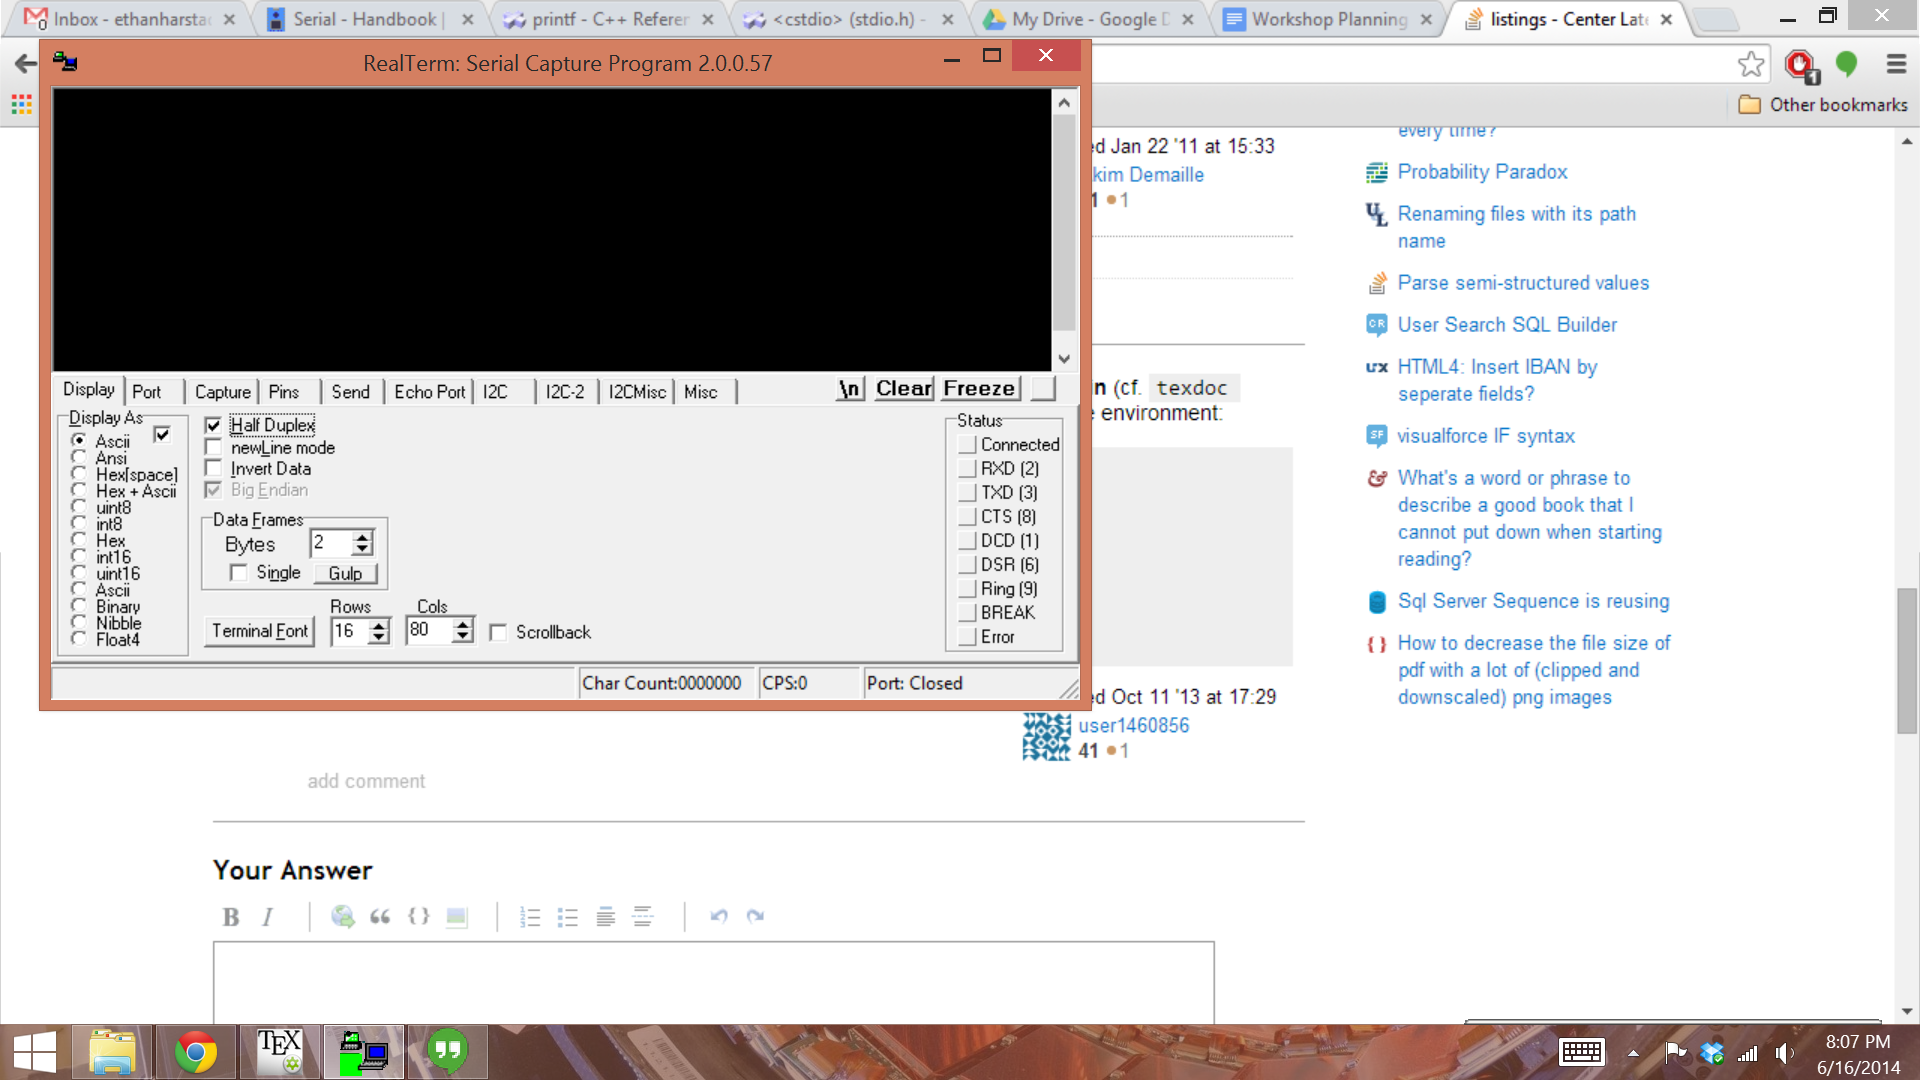
\includegraphics[width=\linewidth]{realterm}
		\end{column}
		\begin{column}{0.5\textwidth}
			\begin{enumerate}
				\item Open RealTerm
				\item Enable "Half Duplex"
				\item Click the "Port" tab
				\item Baud: 9600 and the correct port
				\item Click "Change"
			\end{enumerate}
		\end{column}
	\end{columns}
	\vfill
	Try running a simple sample program:
	\begin{lstlisting}[numbers=none]
		Serial pc(USBTX, USBRX);
		int main() {
		  pc.printf("Hello world!");
		  while(true) {
		    pc.putc(pc.getc() + 1);
		  }
		}
	\end{lstlisting}
\end{frame}

\subsection{Switch/Case Statements}
\label{sub:switch_case}
\begin{frame}[fragile]
	\frametitle{Switch/Case Statements}
	Switch statements can replace some types of if/else statements:
	\begin{columns}[c]
		\begin{column}{0.5\textwidth}
			\begin{lstlisting}[numbers=none]
				switch(variable) {
				  case value1:
				    // Code for value1
				    break;
				  case value2:
				  case value3:
				  	// Code for value2 and 3
				  	break;
				  default:
				    // Code
				}
			\end{lstlisting}
		\end{column}
		\begin{column}{0.5\textwidth}
			\begin{block}{Warning}
				A break statement is required between cases. Forgetting can cause many bugs!
			\end{block}
		\end{column}
	\end{columns}
	Switch statements can only be used with integral type variables.
	You can group multiple cases together like 2 and 3 above.
\end{frame}

\begin{frame}[fragile]
	\frametitle{A New Program}
	\begin{columns}[T]
		\begin{column}{0.5\textwidth}
			Create a new program with:
			\begin{itemize}
				\item A serial port connected to USB
				\item A DigitalOut connected to the LED
				\item A switch statement
				\begin{itemize}
					\item One character turns the LED on
					\item Another character turns the LED off
				\end{itemize}
			\end{itemize}
		\end{column}
		\begin{column}{0.5\textwidth}
			\pause
			\lstinputlisting[caption=RemoteControl.cpp]{code/talking/1.cpp}
		\end{column}
	\end{columns}
\end{frame}

\subsection{Functions}
\label{sub:functions}
\begin{frame}[fragile]
	\frametitle{Functions}
	Functions repackage code into reusable groups:
	\begin{lstlisting}[numbers=none]
		type name(parameter1, parameter2, ...) {statements}
	\end{lstlisting}
	\begin{description}
		\item[type] The type of data returned by the function
		\item[name] The name the function can be called by
		\item[parameters] Variables used as inputs/outputs for the function
		\item[statements] Code statements that define what the function does
	\end{description}
	\vfill
	Parameters are essentially local variable declarations that are passed to the function, use as many (or as few) as needed:
	\begin{lstlisting}[numbers=none]
		int uselessFunction(int a, float b, double c) {...}
	\end{lstlisting}
\end{frame}

\begin{frame}[fragile]
	\frametitle{Using Functions}
	Call a function by using its name and your parameters in parenthesis:
	\begin{lstlisting}[numbers=none]
		int add(int x, int y) {
		  return x + y;
		}
		
		int a = add(2, 3)
		
		a = 5
	\end{lstlisting}
	Some functions do not require a return type:
	\begin{lstlisting}[numbers=none]
		void hello(char * name) {
		  printf("Hello %s\n!", name);
		}
		
		hello("everyone");
		
		>Hello everyone!
	\end{lstlisting}
\end{frame}

\begin{frame}[fragile]
	\frametitle{Revisiting Your Earlier Program}
	\begin{columns}[T]
		\begin{column}{0.5\textwidth}
			Lets rewrite the earlier remote control program to use a function to handle the input.
			This helps us stay organized.\\
			\pause
			\vspace{2ex}
			\textit{Only changed lines are shown to save space}
		\end{column}
		\begin{column}{0.5\textwidth}
	\lstinputlisting[caption=RemoteControl.cpp, firstline=6, firstnumber=6]{code/talking/2.cpp}
		\end{column}
	\end{columns}
\end{frame}

\begin{frame}[fragile]
	\frametitle{Function Prototypes}
	Like variables, functions must be declared before they can be used.\\
	This is why handler was above main in the last example.\\
	\vfill
	You can declare a function prototype separate from the implementation to avoid this:
	\begin{lstlisting}[numbers=none]
		void handler(char in);
		
		int main() { ... }
		
		void handler(char in) { ... }
	\end{lstlisting}
	Put the prototype with the rest of your global declarations and the function where ever it fits best.
\end{frame}

\subsection{For Loops}
\label{sub:for_loops}
\begin{frame}[fragile]
	\frametitle{For Loops}
	For loops execute a block of code a defined number of times:
	\begin{lstlisting}[numbers=none]
		for(initialization; condition; increment) {statements}
	\end{lstlisting}
	\vfill
	\begin{itemize}
		\item Like a while loop, it iterates as long as the condition as true
		\item The initialization statements happens before the first iteration
		\item The increment statement happens after each iteration
	\end{itemize}
	\vfill
	\begin{block}{Example}
		Iterate 10 times, printing the current count:
		\begin{lstlisting}[numbers=none]
			for(int i = 0; i < 10; i++) printf("%d\n", i);
		\end{lstlisting}
	\end{block}
\end{frame}

\begin{frame}[fragile]
	\frametitle{Revisiting Your Earlier Program}
	\begin{columns}[T]
		\begin{column}{0.4\textwidth}
			Edit the remote control program to add a new feature:
			\begin{itemize}
				\item A function to print the abc's using a for loop
				\item A new character in your handler to call your new function
			\end{itemize}
			\pause
		\end{column}
		\begin{column}{0.6\textwidth}
			\lstinputlisting[firstline=15, firstnumber=15]{code/talking/3.cpp}
		\end{column}
	\end{columns}
\end{frame}